\documentclass[a4paper,11pt]{article}

\setlength{\parindent}{0pt}

% Various packages
\usepackage{graphicx}
\usepackage{a4wide}
\usepackage{url}
\usepackage[left=2cm,top=2cm,bottom=1.5cm,right=2cm]{geometry}
\usepackage{amsmath}
\usepackage{amssymb}
\usepackage{amsthm}
\usepackage{amsfonts}
\usepackage{wrapfig}
\usepackage{fixme}
\usepackage{color}
\usepackage{pstricks}
\usepackage{pdfpages}
\usepackage[utf8]{inputenc}
\usepackage{enumitem}
\usepackage{tasks}
\usepackage{float}
\usepackage{dutchcal}

%\usepackage{minted}

\usepackage{listings}
\usepackage{lstautogobble}
\usepackage{semantic}

% Various custom commands
\newcommand{\argmin}{hrm{argmin}}
\newcommand{\R}{\mathbb{R}}
\newcommand{\E}{\mathbb{E}}
\newcommand{\mean}{\mathbb{E}}
\newcommand{\V}{\mathbb{V}}
\newcommand{\prob}{\mathbb{P}}
\newcommand{\var}{\mathrm{var}}
\newcommand{\iid}{\overset{\text{iid}}{\sim}}

\newcommand{\w}{{\mathbf w}}
\newcommand{\x}{{\mathbf x}}
\newcommand{\y}{{\mathbf y}}
\newcommand{\X}{{\mathbf X}}
\renewcommand{\P}[1]{\mathbb P\lrc{#1}}
\DeclareMathAlphabet{\mathpzc}{OT1}{pzc}{m}{it}

\newcommand{\lr}[1]{\left (#1\right)}
\newcommand{\lrc}[1]{{\left \{#1\right\}}}
\newcommand{\lra}[1]{\left |#1\right|}
\newcommand{\lrs}[1]{\left [#1\right]}


\lstset{basicstyle=\ttfamily,
  mathescape=true,
  escapeinside=||,
  autogobble}

\makeatletter
\newcommand*\bigcdot{\mathpalette\bigcdot@{.5}}
\newcommand*\bigcdot@[2]{\mathbin{\vcenter{\hbox{\scalebox{#2}{$\m@th#1\bullet$}}}}}
\makeatother
\usepackage{geometry}
\geometry{
  top=1.3in,    
  inner=1.4in,
  outer=1.4in,
  bottom=1.3in,
  headheight=3ex,  
  headsep=3ex,     
}
\usepackage{fancyhdr}
\pagestyle{fancyplain}
\pagestyle{fancy}
\fancyhf{}
\fancyhead[LE,RO]{Matilde Broløs}
\fancyhead[RE,LO]{PLD - Assignment 3}
\fancyfoot[CE,CO]{}
\fancyfoot[LE,RO]{\thepage}
\renewcommand{\plainheadrulewidth}{0.4pt}

%\usepackage{tikz}


% Making itemized lists that save space
\newenvironment{packed_itemize}{
\begin{itemize}
  \setlength{\itemsep}{1pt}
  \setlength{\parskip}{0pt}
  \setlength{\parsep}{0pt}
}{\end{itemize}}


\title{PLD Assignment 3}
\author{Matilde Broløs (jtw868)}
\date{\today}

\begin{document}

\maketitle

\section*{A3.1}

\subsection*{a)}
The predicate \texttt{writtenIn(M,T)} can be implemented as follows.

\begin{verbatim}
writtenIn(M,program(M)) :-
  program(M).

writtenIn(M,compiler(X, M, Y)) :-
  compiler(X, M, Y).

writtenIn(M,interpreter(X,M)) :-
  interpreter(X,M).
\end{verbatim}

The result of running \texttt{?-writtenIn(M,T)} is seen below.
\begin{figure}[h]
\centering
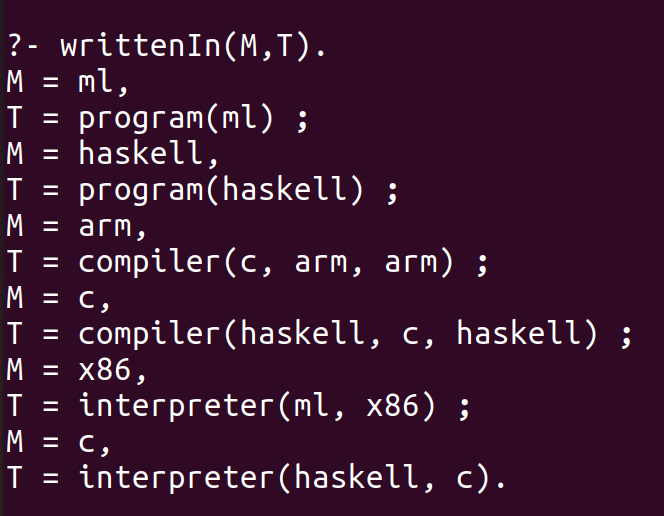
\includegraphics[width=0.5\textwidth]{a31a.png}
\caption{Result of running writtenIn.}
\end{figure}

\subsection*{b)}
The predicate \texttt{canRun(L)} could be implemented as follows.

\begin{verbatim}
canRun(L) :-
  machine(L).

canRun(L) :-
  interpreter(L,X),
  canRun(X).

canRun(L) :-
  compiler(L,X,Y),
  canRun(X),
  canRun(Y).
\end{verbatim}

The result of running \texttt{?-canRun(L)} is seen below.
\begin{figure}[h]
\centering
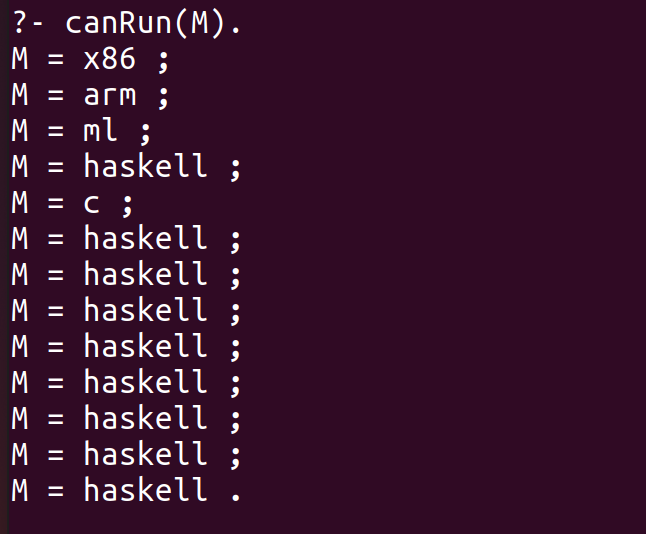
\includegraphics[width=0.5\textwidth]{a31b.png}
\caption{Result of running canRun.}
\end{figure}

\subsection*{c)}
To avoid getting \texttt{L = haskell} an infinite number of times, we add the condition that the compiler cannot translate the program into a new program in the same language. 

\begin{verbatim}
canRun(L) :-
  compiler(L,X,Y),
  L \= Y,
  canRun(X),
  canRun(Y).
\end{verbatim}

Now when running the query we get the following result.
\begin{figure}[h]
\centering
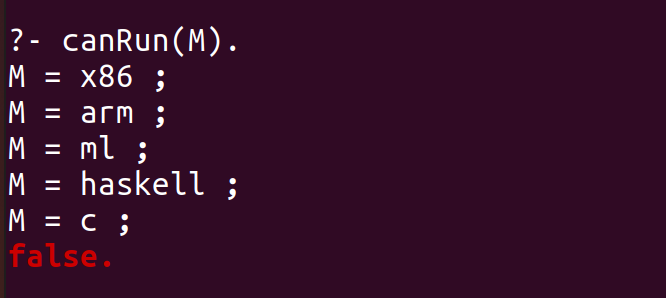
\includegraphics[width=0.5\textwidth]{a31c.png}
\caption{Result of running canRun.}
\end{figure}


\section*{A3.2}

\subsection*{a)}
First lets expand the type system with the rule for the \texttt{let}-expression. First we must check three things:
\begin{enumerate}
	\item When vealuating $e_1$ with an environment $\tau_1$ it evaluates to a type $t_1$
	\item The pattern $p$ matches a type $t_1$ and produces an environment $\tau_2$
	\item When evaluating $e_2$ with an environment $\tau_1 \circ \tau_2$ it evaluates to a type $t_2$
\end{enumerate}
Now if these conditions are true, we can form the \texttt{let}-expression. Thus the final type rule is:
$$\frac{\tau_1 \vdash e_1 : t_1 \; \; \; t_1 \vdash p \hookrightarrow \tau_2 \; \; \; \tau_1 \circ \tau_2 \vdash e_2 : t_2}{\tau \vdash \texttt{let} \; p:t_1 = e_1:t_1 \; \texttt{in} \; e_2:t_2}$$

Now we define the type rules for patterns. If the pattern matches the type \texttt{int} then we produce an empty environment.
$$\frac{}{\texttt{int}\vdash n \hookrightarrow []}$$
If the pattern matches a variable of type $t$ then we map the variable to the type.
$$\frac{}{t\vdash x \hookrightarrow [x \mapsto t]}$$
For the last rule, if $p_1$ is compatible with $t_!$, and $p_2$ is compatible with $t_2$, then the resulting type environment is the two environments combined.
$$\frac{t_1 \vdash p_1 \hookrightarrow \tau_1 \;\;\; t_2 \vdash p_2 \hookrightarrow \tau_2}{(t_1*t_2) \vdash (p_1,p_2) \hookrightarrow \tau_1 \circ \tau_2}$$

\subsection*{b)}
Again we start by writing the semantic rule for the \texttt{let}-expression. The structure follows the same logic as in the previous task.
$$\frac{\rho_1 \vdash e_1 \leadsto v_1 \;\;\; v_1 \vdash p \rightharpoonup \rho_2 \;\;\; \rho_1 \circ \rho_2 \vdash e_2 \leadsto v_2}{\rho \vdash \texttt{let} \;\; p \leadsto v_1 = e_1 \leadsto v_1 \; \texttt{in} \; e_2 \leadsto v_2}$$

Now we define the semantic rules for patterns. If $v=n$, where $n$ is a number, then when $v$ matches $n$ we produce the empty value environment.
$$\frac{v=n}{v\vdash n \rightharpoonup []}$$
When the pattern is a variable $x$ matching a value $v$, the produced environment maps the variable to the value $v$.
$$\frac{}{v \vdash x \rightharpoonup [x \mapsto v]}$$
Last last rule follows the logic of the type system rule very closely. If the pattern $p_1$ matches a value $v_1$ and produces an environment $\rho_1$, and the pattern $p_2$ matches a value $v_2$ and produces an environment $\rho_2$, then the environment of the pair of the two patterns will be the two environments combined.
$$\frac{v_1 \vdash p_1 \rightharpoonup \rho_1 \;\;\; v_2 \vdash p_2 \rightharpoonup \rho_2}{(v_1*v_2)\vdash (p_1,p_2) \rightharpoonup \rho_1 \circ \rho_2}$$

\section*{A3.3}

\subsection*{a)}
The probability that the third-largest of 39 nine-sided dice will be 8 can be calculated with the following command in Troll.

\begin{verbatim}
least 1 largest 3 39d9
\end{verbatim}

The result can be seen in figure \ref{fig:troll}.

\begin{figure}[h]
\centering
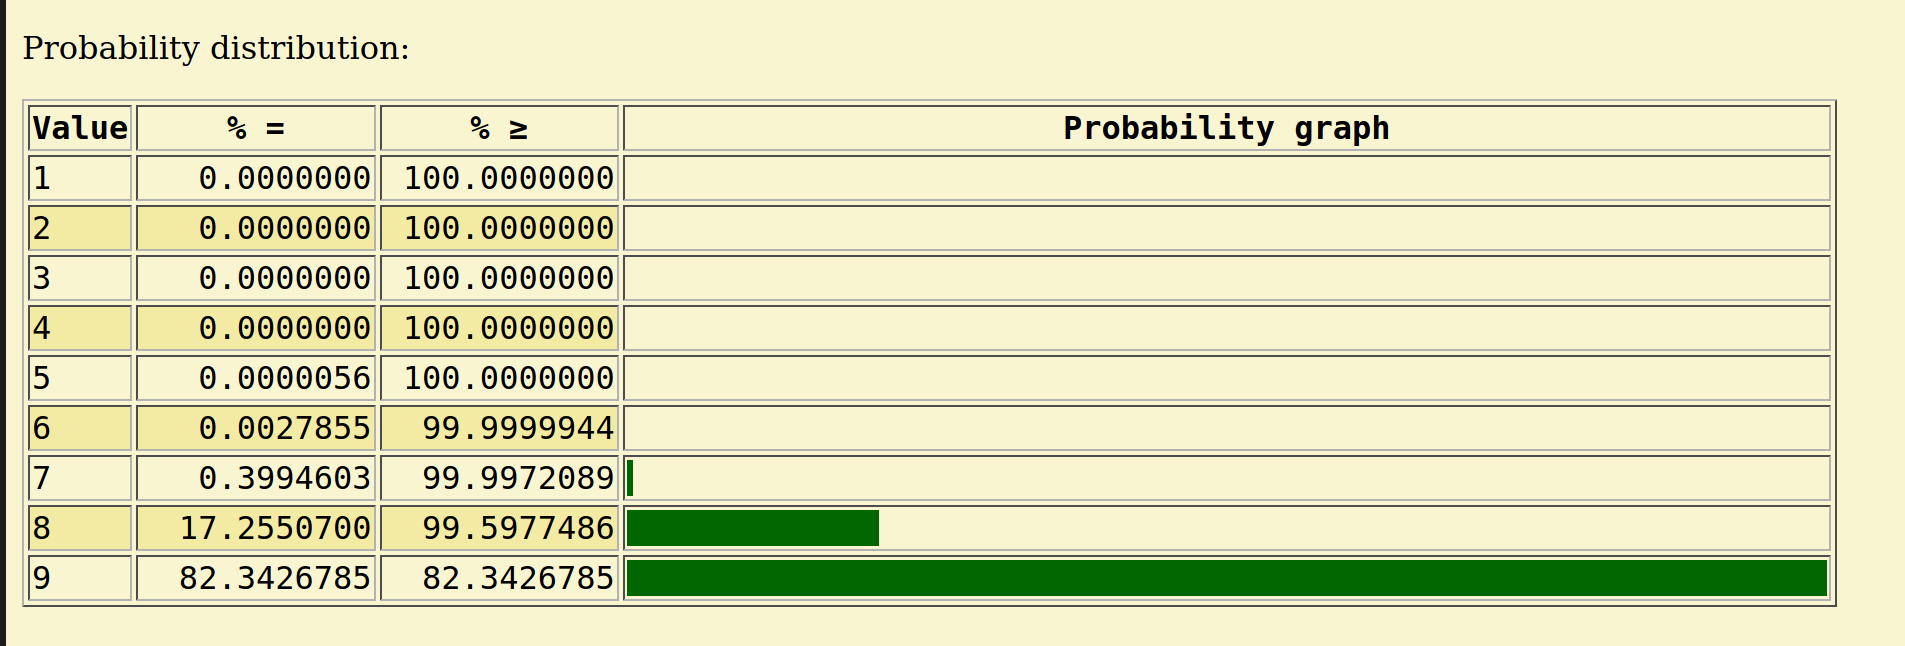
\includegraphics[width=0.8\textwidth]{a33a.png}
\caption{Result of running the above code.}
\label{fig:troll}
\end{figure}

Thus, the probability is $0.172550700$.

\subsection*{b)}
To compute the probability of $8$ being the third highest roll when rolling $39$ $9$-sided dice, lets first look at the first three rolls. There are a number of different combinations of numbers in the first three rolls. Lets represent any $8$'s by $e$ and $9$'s by $n$, and all other values by $x$. Now the first thing the program should do is calculate the probabilities of the different throws. I chose to write this program in python, and this first calculation is shown below.

\begin{verbatim}
# Number of rolls and sides on dice
die_rolls = 39
die_sides = 9

# Probability that result is lower than 8
lo_prob = (7 / die_sides)
# Probability that result a specific roll, here either 8 or 9
hi_prob = (1 / die_sides)

# Cases for the first 3 dice. 'e' is for 8, 'n' is for 9, and 'x' is for 1-7.
# The probability of the case is multiplied by the number of permutations.

# All cases where neither 8 nor 9 is included
xxx = ((7**3) / (9**3))
# Cases xx8 x8x 8xx
exx = (lo_prob**2 * hi_prob) * 3
# Cases xx9 x9x 9xx
nxx = (lo_prob**2 * hi_prob) * 3
# Cases 88x 8x8 x88
eex = (lo_prob * hi_prob**2) * 3
# Cases 99x 9x9 x99
nnx = (lo_prob * hi_prob**2) * 3
# Cases 98x 89x 8x9 9x8 x89 x98
nex = (lo_prob * hi_prob**2) * 6
# Cases 998 989 899
nne = (hi_prob**3) * 3
# Cases 889 898 988
nee = (hi_prob**3) * 3
# Case 888
eee = hi_prob**3
\end{verbatim}

Now we have the probability for each of these combinations, and we need to add the remaining $36$ rolls. For each roll we update the probability for each of the above cases, thus for example the probability that \texttt{xxx} remains the hghest three dice is equal to the current possibility times \texttt{lo\_prob}, as we need to count the cases where the new die is neither $8$ nor $9$.

The code for this is presented below.

\begin{verbatim}
for i in range(die_rolls - 3):
    tmp_xxx = xxx * lo_prob
    tmp_exx = (exx * lo_prob) + (xxx * hi_prob)
    tmp_nxx = (nxx * lo_prob) + (xxx * hi_prob)
    tmp_eex = (eex * lo_prob) + (exx * hi_prob)
    tmp_nnx = (nnx * lo_prob) + (nxx * hi_prob)
    tmp_nex = (nex * lo_prob) + (nxx * hi_prob) + (exx * hi_prob)
    tmp_eee = (eee * lo_prob) + (eex * hi_prob) + (eee * hi_prob)
    tmp_nne = (nne * lo_prob) + (nne * hi_prob) + (nee * hi_prob)
                              + (nex * hi_prob) + (nnx * hi_prob)
    tmp_nee = (nee * lo_prob) + (nee * hi_prob) + (eee * hi_prob)
                              + (nex * hi_prob) + (eex * hi_prob)
    xxx = tmp_xxx
    exx = tmp_exx
    nxx = tmp_nxx
    eex = tmp_eex
    nnx = tmp_nnx
    nex = tmp_nex
    eee = tmp_eee
    nne = tmp_nne
    nee = tmp_nee


# Print the result with 9 decimals
print("The probability is %.9f" % (eee + nee + nne))
\end{verbatim}

When running this code, we get that the probability is $0.172550700$ which is precisely equal to the result we got from the Troll code.


\subsection*{c)}
The size of the Python program is remarkably bigger than the Troll program, and it was much more difficult to write. The length of the program also decreases understandability, as it is not immediately clear what the code does. When understanding the syntax of Troll, the program was easy to write, and easy for the reader to understand as well. 
Furthermore, the Troll program can easily be modified to calculate a different number of rolls, or different number of largest rolls. The python progam, on the other hand, can relatively easily be change to compute a different number of rolls, but to change it to a different number of largest rolls would not be easy.
Concerning runtime, it seems that both programs compute the result very fast, at least when dealing with such a small calculation as this.


\end{document}
